% !Mode:: "TeX:UTF-8"
% !TEX root = ..\thesis.tex
\chapter{绪论}
\section{课题研究的背景及意义}

汽车装配大多采用同步装配流水线方式作业,将装配过程分为多个作业单元,并安排在流水线的相应工位上。然而,随着技术的日新月异,客户需求的多样化,以及精益思想、环保节能观念的出现,汽车工业的生产模式不得不转变为面向订单的大批量、多品种的生产方式,这使得汽车电子部件的装配生产也要呈现多品种与批量化,以配合汽车生产。因此,缩短交货期、提高资源利用率、降低生产成本、提高生产运作的灵活性,已成为保证企业市场竞争力的重要手段。

多品种装配是在基本不改变或较少改变现有生产设施的前提下,通过对装配生产线的合理组织与调度优化,实现多品种共线装配,以最大限度地挖掘生产线的潜能,向客户提供定制的个性化产品和服务。

生产调度就是组织执行生产进度计划的工作,作为一种决策形式,调度在制造业扮演者至关重要的角色,尤其在现今充满竞争的环境下,有效的生产调度已成为能在市场竞争下生存的必须。

从上个世纪50年代起,调度问题的研究就受到应用数学、运筹学、工程技术等领域科学家的重视,科学家们利用运筹学中的线性规划、整数规划、目标规划、动态规划及决策分析方法,研究并解决了一系列有代表意义的调度和优化问题\cite{徐俊刚2004}。如今,随着计算机的发展,信息技术的成熟,许多过去只在理论层面上的调度算法,都可以通过计算机辅助得以验证与运用,给制造业的具体实力提升带来了可能。

提高竞争力的方法有很多,对于汽车工业,产品需求多样化和市场细分化,促使越来越多的制造商将多品种装配作为增强其竞争能力的有效手段。因此,合理安排装配产线,优化调度作业单元,对保证汽车电子部件装配质量,快速响应需求,提高汽车电子部件装配线的生产效率有着重要的现实意义。

举例来说,随着调度问题的规模增大,人们发现即使通过计算机,有些问题的算法并不是有效的,因为它们的求解超出了可接受的运行时间。逻辑学家和计算机科学家通过研究这类问题,建立了复杂度理论,并称这些问题是$NP$问题,问题的复杂度是会随着问题规模增大呈现指数爆炸。

这样一来,有时得到最优调度或者最优解的成本就变得太高了,那么近似最优解便成了很好的选择。然而调度问题的算法本来就众多,求解近似最优解更是如此,不同的算法适用的情况也不尽相同。实践表明,寻找合适的调度方案对生产系统的运行有着显著的影响。因此,从多品种装配着手研究调度算法,对增加产品多样性,加快需求响应速度,加快提高企业的竞争力有着重要意义。


\section{国内外研究现状}
调度问题本身具有高复杂性、多约束性、多目标性,在多品种大批量生产方式下,由于产品品种多、批量大、零件多等特点,增加了调度的复杂程度。多品种的装配调度问题是一种常见的车间调度问题,对于汽车零件,又有其独有的工艺特点。所以研究这个问题需要从调度规则、目标确定、工艺过程、设施类型等方面入手,提出合适的算法。

有关调度问题的算法研究颇多,而且随着目标函数的不同及目标数量的增多而逐渐呈现多元化,与之而来的便是难度增大,几乎不可能得到最优解,但是,许多$NP - Hard$问题还是相继得到解决。近来的研究热点以启发式算法为主,并呈现多种方法结合使用的趋势。

对于多品种调度的研究,国内外学者在调度的算法改造中有很多创新,在其研究的课题中体现出优良的性能,实用价值很大,对本课题的算法研究启发颇多。

将产品分类或者确定产品簇,这在多品种的装配问题来说很重要。
Xie Zhiqiang\cite{xie2010study} 等通过建立虚拟产品,将多品种问题转化为单品种问题,通过关键路径方法确定加工顺序后,根据各工位操作的特征运用不同的算法调度,然后进行整合,解决了单产品的柔性调度,最后添加作业间的约束,较好的解决了复杂的多品种调度问题,对于简单的多品种调度问题,甚至可以不用加入作业间的约束。
唐勇智\cite{唐勇智2009基于聚类的}通过研究RBF-LBF 串联神经网络,改进K-means 聚类算法,提出了自适应的SA-K-means 算法,本课题的研究可以借鉴其思想,更为有效的将产品簇分类。
陈伟\cite{陈伟2006生物信息学中的序列相似性比对算法}通过Smith-Waterman, FASTA 和BLAST 三个局部对比算法,较好的找到了相似性较高的DNA 序列,对于本课题中的产品簇归类有很高的借鉴意义。

有关建模设计的研究众多,主要是有关目标函数与约束的建立,
李斌\cite{李斌2009}等提出了车间调度Multi-Agent 模型,以延期成本、设备利用率、综合调度性能等指标作为目标函数,并通过Lekin 软件和实例比较了不同调度规则下的效果。
M.A. Adibi\cite{adibi2010multi}等研究了随机作业和有机器抛锚可能的动态作业车间调度问题,通过经学习的神经网络,更新变邻域搜索算法的参数,在常见的分配规则下,较好的解决了该目标包括制造期和延迟的调度问题,并且其适用范围很广,其特点是神经网络的应用,很大程度上提高了搜索性能。
刘文平\cite{刘文平2009}将汽车装配的多种订单产品序列优化看作约束满足的调度模型,通过邻域搜索算法中的Memetic 算法,优化了混合品种装配线调度。
杨本强\cite{杨本强2002}运用线性规划理论,建立了汽车流水线均衡生产模型,并通过一个启发式搜索算法来探寻解,思路简单,容易实现,本课题的微观调整可以借鉴其思想。
李宏霞\cite{李宏霞2006}等载荷考虑了物料配送能力,运用FCFS 规则的相关算法\cite{lo2002job}提出了一种操作性较强的调度模型,较好的解决了多品种变批量的装配调度问题。
B.J.V. da Silva\cite{da2014production} 等通过航空行业的实例研究,考虑了人力的水平等级,学习影响及作业空间的限制,将飞机装配分成4个不同程度的阶段,各阶建立或增改约束模型,有效解决了含有邻接约束的装配调度问题。
A. Tharumarajah\cite{1998distributed}等考虑了基于行为的分布式控制,并将之用于装配调度模型中,有效地解决了一个3阶段4工作站的装配问题,与整数规划相比,基于行为的调度无论在运行时间或是适用规模上,都显著优于整数规划。
李志娟\cite{李志娟2008}等通过研究高校排课问题,在有效、交错、分散、固定、优先的原则下,设计了一个基于规则的算法,并在产生冲突时进行回溯,得到较好的课程表,其设计思想可以用到本课题中,有其是在多种目标下,设计相应的规则算法。
P. Chutima\cite{chutima2014pareto}等考虑了学习因子,提出了基于生物地域最优方法的方法,应用于两边装配线的混合模型,并引入了适应性机制,化解了最小化生产变化率、最小化总时间利用率、最小化调度序列换线时间三个矛盾,并使它们同时最优,提高了该元启发式方法的性能,有效的解决了多样性装配的调度。

在解的搜索上,启发式方法在搜索局部最优时效果很好,而涉及到全局最优就需要考虑元启发算法。
陈琳\cite{陈琳2009}等将其撤装配车间简化成一个流水车间问题,并通过改进得到带有记忆的模拟退火算法,并引入禁忌搜索机制得到较好的近似最优解。
台湾学者Ham-Huah Hsu\cite{hsu1995fully}等研究了多机器人的装配单元,通过基于搜索算法的调度,并将之仿真。
Jia Shuai\cite{jia2014path} 等通基于禁忌搜索算法,通过路线重建和回跳追踪方法进行排序决策,解决了多目标的柔性作业车间调度问题。
G. Moslehi\cite{moslehi2011pareto}等研究了柔性作业车间,提出了结合蚁群算法和邻域搜索算法的方法,解决了多目标的作业车间调度问题,得到了质量较高,计算时间合理的近似最优解,尤其在中、大型问题中更能体现优势,并且该方法的提升空间很大。
台湾学者Rock Lin\cite{lin2012case}等通过峰明机械厂的案例研究,引入作业划分概念和批量处理,提出了一个混合整数规划模型和3个启发式方法FBEDD、FBFS、RFBFS ,并通过计算实验证明FBEDD 在解决小型问题上较好,而对于中大型的问题,RFBFS 便具有更好的求解结果。
朱有产\cite{朱有产2006}等通过改进经典的Dijkstra 搜索算法,引入空间向量,通过夹角参数,有效的快速跳出局部最优解,得到最短路径问题的全局最优,对本课题的解的搜索有启发意义,可以将之结合入粒子群算法,重新定义其方向参数以改进。
高丽\cite{高丽2012}等基于精英选择和个体迁移的多目标方法对遗传算法改进,得到了较好的多品种生产调度的Pareto 解集。
曹洪鑫\cite{曾洪鑫2006}等将多品种产品的混流装配顺序看作是商旅问题(TSP),其加工和换模时间即转化为路程,并通过遗传算法进行了100次迭代,较好的找到了较优解。本课题主要研究对象虽然不是混流装配,但混线时可以用到这个想法。讲到(TSP),翁武熙\cite{翁武熙2012混合蚁群算法求解}采用了结合蛙跳算法的新型智能算法,较好的改进了蚁群算法的搜索过程,值得借鉴。


\section{课题的研究内容及技术路线}
根据实际调研和国内外研究现状,针对该厂汽车装配目前存在的一些问题和不足,提出以下研究内容:
\renewcommand{\labelenumi}{(\theenumi)}
\begin{asparaenum}
\item 生产线调度现状分析
\suspend{asparaenum}

这部分为汽车电子零部件多品种多装配线生产的调研,分析当前生产过程,找出可以改进的地方,并提出改进方案。
\resume{asparaenum}
\item 构建调度模型
\suspend{asparaenum}

根据企业的订单到达稳定情况,可以建立不同的模型。结合产品簇的分类和实际情况,确定有效的目标函数,在可接受的假设条件下设置相关约束构,建合理的调度模型。其中目标函数的确定即要考虑实际生产,又要兼顾求解的过程。
\resume{asparaenum}
\item 模型求解和算法实现
\suspend{asparaenum}

通过有效的求解算法获得初始解及搜索算法以改进初始解,算法的设计主要考虑可以在合理的时间内实现,并能得到最优或者质量较高的局部最优解。
\resume{asparaenum}
\item 计算实验
\end{asparaenum}

计算实验的设计可以对所提模型进行求解,并比较不同算法下的改进效果。

装配车间调度的关键技术是和调度相关的技术,需要有调度理论的框架和相关概念,
本课题以某汽车电子公司的装配车间为对象,对多品种的调度安排进行研究。首先对产线生产现状分析,提出改进方案,根据方案建立相应调度的数学模型。然后根据模型的特征,设计求解算法,并通过计算实验评估算法的性能,提出该算法在调度实践的意义。

%除了调度的结构体系,其实现算法也相当关键,和本研究的相关算法中,选取3个具有代表的:完整批产品簇排序(FBFS)、变领域搜索(VNS)和粒子群优化算法(PSO)。FBFS 算法的特点是将作业按簇分成批次,可以有效减少作业簇准备时间,适合多品种的生产调度,这是直接从调度本身入手的,可操作性很大,而且较符合实用情况,虽然有其不完善,但改善比较容易。VNS 和PSO 都是解的搜索方法,理论性较强,可以将两者结合实用,比如在VNS 随机下一个领域的的阶段可以通过PSO 来确定下一个搜索方向,发挥两者的优势。只是仅从目标函数的解空间搜索,获得的结果可能会在实用中出现相关问题,需要进一步通过实践研究。

本课题采用的基本思路和关键技术路线如\reff{fig:1}所示。
\begin{figure}[h]
\centering
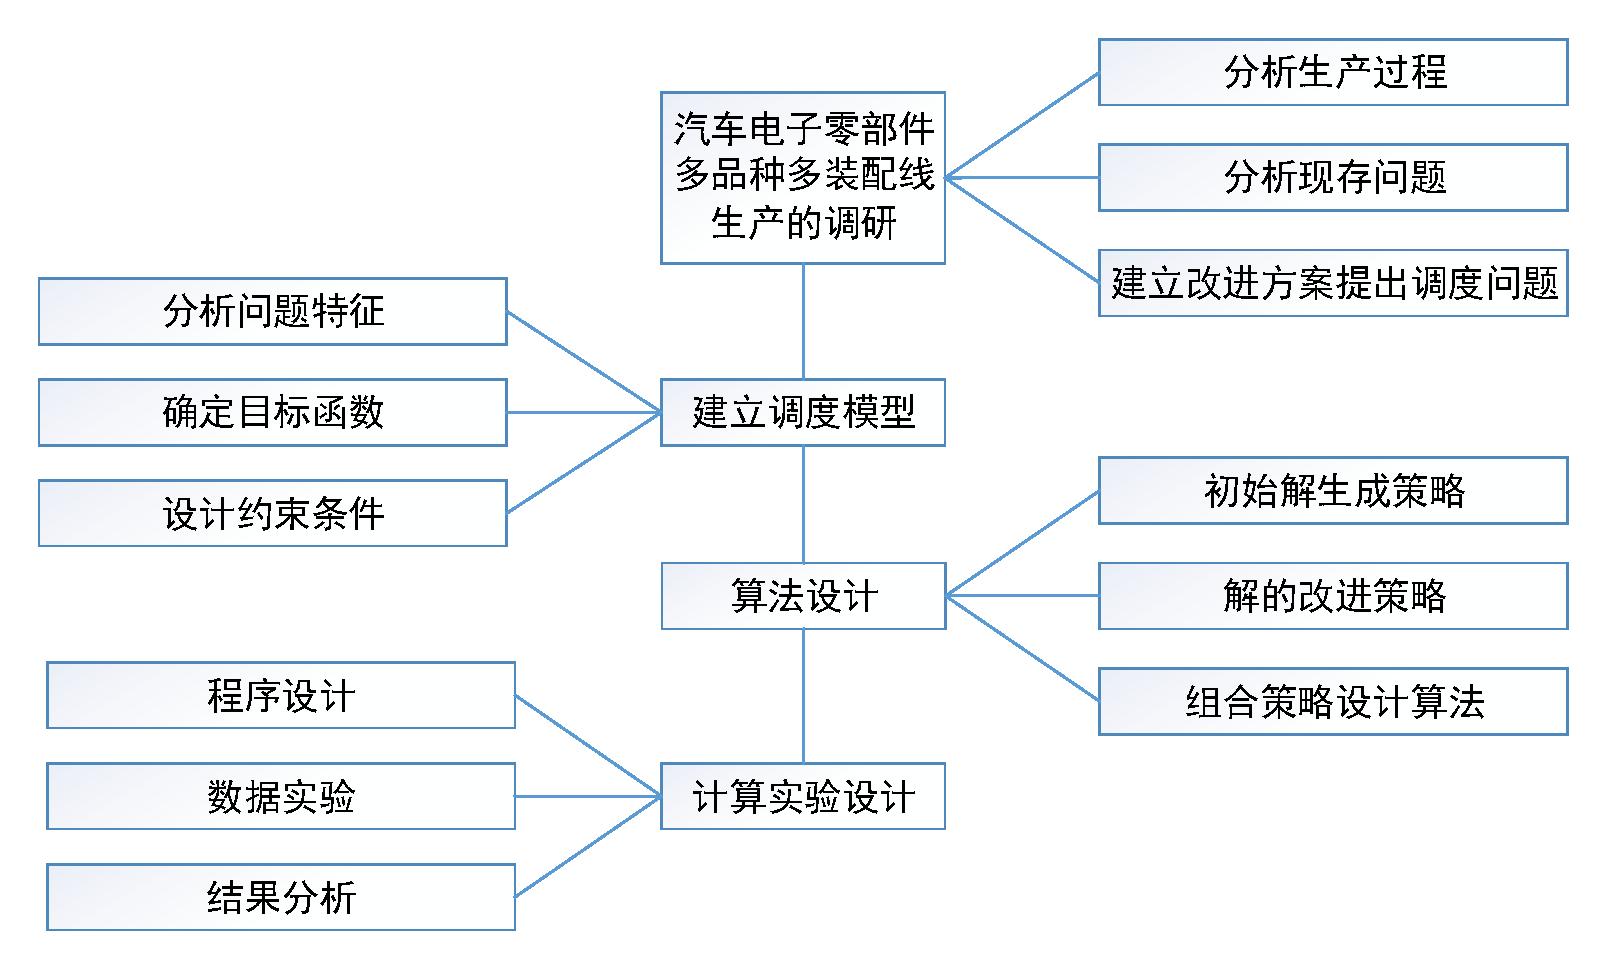
\includegraphics[width = 15cm]{techroute1.pdf}
\caption{基本思路和关键技术路线\label{fig:1}}
\end{figure}